% Options for packages loaded elsewhere
\PassOptionsToPackage{unicode}{hyperref}
\PassOptionsToPackage{hyphens}{url}
%
\documentclass[
  ignorenonframetext,
]{beamer}
\usepackage{pgfpages}
\setbeamertemplate{caption}[numbered]
\setbeamertemplate{caption label separator}{: }
\setbeamercolor{caption name}{fg=normal text.fg}
\beamertemplatenavigationsymbolsempty
% Prevent slide breaks in the middle of a paragraph
\widowpenalties 1 10000
\raggedbottom
\setbeamertemplate{part page}{
  \centering
  \begin{beamercolorbox}[sep=16pt,center]{part title}
    \usebeamerfont{part title}\insertpart\par
  \end{beamercolorbox}
}
\setbeamertemplate{section page}{
  \centering
  \begin{beamercolorbox}[sep=12pt,center]{part title}
    \usebeamerfont{section title}\insertsection\par
  \end{beamercolorbox}
}
\setbeamertemplate{subsection page}{
  \centering
  \begin{beamercolorbox}[sep=8pt,center]{part title}
    \usebeamerfont{subsection title}\insertsubsection\par
  \end{beamercolorbox}
}
\AtBeginPart{
  \frame{\partpage}
}
\AtBeginSection{
  \ifbibliography
  \else
    \frame{\sectionpage}
  \fi
}
\AtBeginSubsection{
  \frame{\subsectionpage}
}
\usepackage{amsmath,amssymb}
\usepackage{lmodern}
\usepackage{iftex}
\ifPDFTeX
  \usepackage[T1]{fontenc}
  \usepackage[utf8]{inputenc}
  \usepackage{textcomp} % provide euro and other symbols
\else % if luatex or xetex
  \usepackage{unicode-math}
  \defaultfontfeatures{Scale=MatchLowercase}
  \defaultfontfeatures[\rmfamily]{Ligatures=TeX,Scale=1}
\fi
% Use upquote if available, for straight quotes in verbatim environments
\IfFileExists{upquote.sty}{\usepackage{upquote}}{}
\IfFileExists{microtype.sty}{% use microtype if available
  \usepackage[]{microtype}
  \UseMicrotypeSet[protrusion]{basicmath} % disable protrusion for tt fonts
}{}
\makeatletter
\@ifundefined{KOMAClassName}{% if non-KOMA class
  \IfFileExists{parskip.sty}{%
    \usepackage{parskip}
  }{% else
    \setlength{\parindent}{0pt}
    \setlength{\parskip}{6pt plus 2pt minus 1pt}}
}{% if KOMA class
  \KOMAoptions{parskip=half}}
\makeatother
\usepackage{xcolor}
\IfFileExists{xurl.sty}{\usepackage{xurl}}{} % add URL line breaks if available
\IfFileExists{bookmark.sty}{\usepackage{bookmark}}{\usepackage{hyperref}}
\hypersetup{
  pdftitle={Pearson and the crabs from Naples bay},
  hidelinks,
  pdfcreator={LaTeX via pandoc}}
\urlstyle{same} % disable monospaced font for URLs
\newif\ifbibliography
\usepackage{color}
\usepackage{fancyvrb}
\newcommand{\VerbBar}{|}
\newcommand{\VERB}{\Verb[commandchars=\\\{\}]}
\DefineVerbatimEnvironment{Highlighting}{Verbatim}{commandchars=\\\{\}}
% Add ',fontsize=\small' for more characters per line
\usepackage{framed}
\definecolor{shadecolor}{RGB}{248,248,248}
\newenvironment{Shaded}{\begin{snugshade}}{\end{snugshade}}
\newcommand{\AlertTok}[1]{\textcolor[rgb]{0.94,0.16,0.16}{#1}}
\newcommand{\AnnotationTok}[1]{\textcolor[rgb]{0.56,0.35,0.01}{\textbf{\textit{#1}}}}
\newcommand{\AttributeTok}[1]{\textcolor[rgb]{0.77,0.63,0.00}{#1}}
\newcommand{\BaseNTok}[1]{\textcolor[rgb]{0.00,0.00,0.81}{#1}}
\newcommand{\BuiltInTok}[1]{#1}
\newcommand{\CharTok}[1]{\textcolor[rgb]{0.31,0.60,0.02}{#1}}
\newcommand{\CommentTok}[1]{\textcolor[rgb]{0.56,0.35,0.01}{\textit{#1}}}
\newcommand{\CommentVarTok}[1]{\textcolor[rgb]{0.56,0.35,0.01}{\textbf{\textit{#1}}}}
\newcommand{\ConstantTok}[1]{\textcolor[rgb]{0.00,0.00,0.00}{#1}}
\newcommand{\ControlFlowTok}[1]{\textcolor[rgb]{0.13,0.29,0.53}{\textbf{#1}}}
\newcommand{\DataTypeTok}[1]{\textcolor[rgb]{0.13,0.29,0.53}{#1}}
\newcommand{\DecValTok}[1]{\textcolor[rgb]{0.00,0.00,0.81}{#1}}
\newcommand{\DocumentationTok}[1]{\textcolor[rgb]{0.56,0.35,0.01}{\textbf{\textit{#1}}}}
\newcommand{\ErrorTok}[1]{\textcolor[rgb]{0.64,0.00,0.00}{\textbf{#1}}}
\newcommand{\ExtensionTok}[1]{#1}
\newcommand{\FloatTok}[1]{\textcolor[rgb]{0.00,0.00,0.81}{#1}}
\newcommand{\FunctionTok}[1]{\textcolor[rgb]{0.00,0.00,0.00}{#1}}
\newcommand{\ImportTok}[1]{#1}
\newcommand{\InformationTok}[1]{\textcolor[rgb]{0.56,0.35,0.01}{\textbf{\textit{#1}}}}
\newcommand{\KeywordTok}[1]{\textcolor[rgb]{0.13,0.29,0.53}{\textbf{#1}}}
\newcommand{\NormalTok}[1]{#1}
\newcommand{\OperatorTok}[1]{\textcolor[rgb]{0.81,0.36,0.00}{\textbf{#1}}}
\newcommand{\OtherTok}[1]{\textcolor[rgb]{0.56,0.35,0.01}{#1}}
\newcommand{\PreprocessorTok}[1]{\textcolor[rgb]{0.56,0.35,0.01}{\textit{#1}}}
\newcommand{\RegionMarkerTok}[1]{#1}
\newcommand{\SpecialCharTok}[1]{\textcolor[rgb]{0.00,0.00,0.00}{#1}}
\newcommand{\SpecialStringTok}[1]{\textcolor[rgb]{0.31,0.60,0.02}{#1}}
\newcommand{\StringTok}[1]{\textcolor[rgb]{0.31,0.60,0.02}{#1}}
\newcommand{\VariableTok}[1]{\textcolor[rgb]{0.00,0.00,0.00}{#1}}
\newcommand{\VerbatimStringTok}[1]{\textcolor[rgb]{0.31,0.60,0.02}{#1}}
\newcommand{\WarningTok}[1]{\textcolor[rgb]{0.56,0.35,0.01}{\textbf{\textit{#1}}}}
\usepackage{longtable,booktabs,array}
\usepackage{calc} % for calculating minipage widths
\usepackage{caption}
% Make caption package work with longtable
\makeatletter
\def\fnum@table{\tablename~\thetable}
\makeatother
\usepackage{graphicx}
\makeatletter
\def\maxwidth{\ifdim\Gin@nat@width>\linewidth\linewidth\else\Gin@nat@width\fi}
\def\maxheight{\ifdim\Gin@nat@height>\textheight\textheight\else\Gin@nat@height\fi}
\makeatother
% Scale images if necessary, so that they will not overflow the page
% margins by default, and it is still possible to overwrite the defaults
% using explicit options in \includegraphics[width, height, ...]{}
\setkeys{Gin}{width=\maxwidth,height=\maxheight,keepaspectratio}
% Set default figure placement to htbp
\makeatletter
\def\fps@figure{htbp}
\makeatother
\setlength{\emergencystretch}{3em} % prevent overfull lines
\providecommand{\tightlist}{%
  \setlength{\itemsep}{0pt}\setlength{\parskip}{0pt}}
\setcounter{secnumdepth}{-\maxdimen} % remove section numbering
\ifLuaTeX
  \usepackage{selnolig}  % disable illegal ligatures
\fi

\title{Pearson and the crabs from Naples bay}
\author{}
\date{\vspace{-2.5em}}

\begin{document}
\frame{\titlepage}

\begin{frame}{Section header (Slide 2)}
\protect\hypertarget{section-header-slide-2}{}
In 1892, Weldon and his wife collected extensive data on populations of
the crab, Carcinus Moenas, and observed that one trait, the forehead
width to the body length ratio, in the crabs from Naples bay actually
showed a highly skewed, rather than a normal, distribution.

Weldon wondered whether this distribution could be the result of the
population being a mix of two different normal distributions, with the
possible implication that the population consisted of two different
races or `types' in the same locality.
\end{frame}

\begin{frame}{}
\protect\hypertarget{section}{}
\begin{figure}
\centering
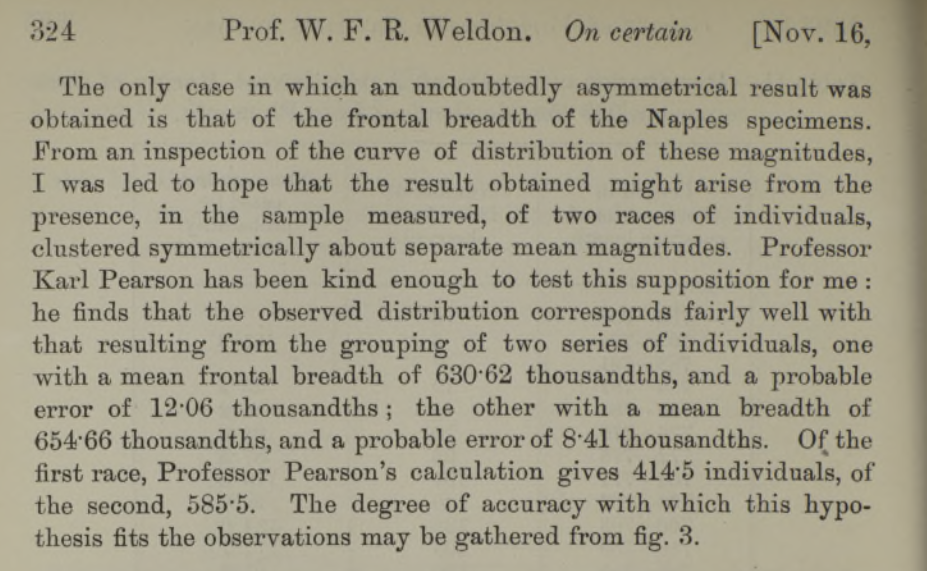
\includegraphics{weldon_paper.png}
\caption{lr}
\end{figure}

\href{normal.png}{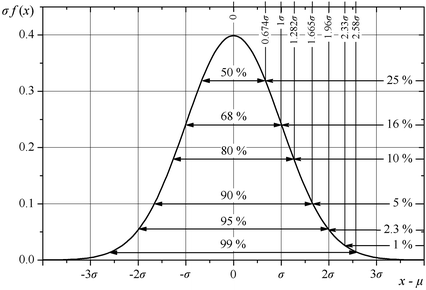
\includegraphics{normal.png}}
\end{frame}

\begin{frame}{}
\protect\hypertarget{section-1}{}
\end{frame}

\begin{frame}{Section header (Slide 2)}
\protect\hypertarget{section-header-slide-2-1}{}
\begin{figure}

\includegraphics{pearsonnb_files/figure-beamer/unnamed-chunk-1-1} \hfill{}

\caption{The horizontal scale represents thousandths of the carapace length, the vertical scale numbers of individuals. Each ordinate of the upperdotted curve is the sum of the corresponding ordinates of the two componentcurves.}\label{fig:unnamed-chunk-1}
\end{figure}
\end{frame}

\begin{frame}{}
\protect\hypertarget{section-2}{}
\end{frame}

\begin{frame}{}
\protect\hypertarget{section-3}{}
\end{frame}

\begin{frame}{Dataset}
\protect\hypertarget{dataset}{}
\begin{columns}[T]
\begin{column}{0.48\textwidth}
\begin{longtable}[]{@{}rr@{}}
\toprule
ratio & freq \\
\midrule
\endhead
0.5835 & 1 \\
0.5875 & 3 \\
0.5915 & 5 \\
0.5955 & 2 \\
0.5995 & 7 \\
0.6035 & 10 \\
0.6075 & 13 \\
0.6115 & 19 \\
\bottomrule
\end{longtable}
\end{column}

\begin{column}{0.48\textwidth}
\begin{longtable}[]{@{}lrr@{}}
\toprule
& ratio & freq \\
\midrule
\endhead
9 & 0.6155 & 20 \\
10 & 0.6195 & 25 \\
11 & 0.6235 & 40 \\
12 & 0.6275 & 31 \\
13 & 0.6315 & 60 \\
14 & 0.6355 & 62 \\
15 & 0.6395 & 54 \\
16 & 0.6435 & 74 \\
17 & 0.6475 & 84 \\
\bottomrule
\end{longtable}
\end{column}
\end{columns}
\end{frame}

\begin{frame}[fragile]{}
\protect\hypertarget{section-4}{}
\includegraphics{pearsonnb_files/figure-beamer/unnamed-chunk-3-1.pdf}

\begin{verbatim}
##     ratio freq
## 1  0.5835    1
## 2  0.5875    3
## 3  0.5915    5
## 4  0.5955    2
## 5  0.5995    7
## 6  0.6035   10
## 7  0.6075   13
## 8  0.6115   19
## 9  0.6155   20
## 10 0.6195   25
## 11 0.6235   40
## 12 0.6275   31
## 13 0.6315   60
## 14 0.6355   62
## 15 0.6395   54
## 16 0.6435   74
## 17 0.6475   84
## 18 0.6515   86
## 19 0.6555   96
## 20 0.6595   85
## 21 0.6635   75
## 22 0.6675   47
## 23 0.6715   43
## 24 0.6755   24
## 25 0.6795   19
## 26 0.6835    9
## 27 0.6875    5
## 28 0.6915    0
## 29 0.6955    1
\end{verbatim}

\begin{verbatim}
##      ratio             freq      
##  Min.   :0.5835   Min.   : 0.00  
##  1st Qu.:0.6115   1st Qu.: 7.00  
##  Median :0.6395   Median :24.00  
##  Mean   :0.6395   Mean   :34.48  
##  3rd Qu.:0.6675   3rd Qu.:60.00  
##  Max.   :0.6955   Max.   :96.00
\end{verbatim}
\end{frame}

\begin{frame}[fragile]{}
\protect\hypertarget{section-5}{}
\includegraphics{pearsonnb_files/figure-beamer/unnamed-chunk-4-1.pdf}

\begin{verbatim}
##        ratio  specie    ratioj
##    1: 0.5855 unknown 0.5855633
##    2: 0.5895 unknown 0.5910523
##    3: 0.5895 unknown 0.5892707
##    4: 0.5895 unknown 0.5913135
##    5: 0.5935 unknown 0.5942331
##   ---                         
##  996: 0.6895 unknown 0.6896138
##  997: 0.6895 unknown 0.6909158
##  998: 0.6895 unknown 0.6888823
##  999: 0.6895 unknown 0.6894942
## 1000: 0.6975 unknown 0.6976330
\end{verbatim}

\begin{verbatim}
##      ratio           specie              ratioj      
##  Min.   :0.5855   Length:1000        Min.   :0.5856  
##  1st Qu.:0.6375   Class :character   1st Qu.:0.6364  
##  Median :0.6495   Mode  :character   Median :0.6512  
##  Mean   :0.6487                      Mean   :0.6487  
##  3rd Qu.:0.6615                      3rd Qu.:0.6623  
##  Max.   :0.6975                      Max.   :0.6976
\end{verbatim}

\begin{verbatim}
## [1] 0.01910579
\end{verbatim}
\end{frame}

\begin{frame}[fragile]{}
\protect\hypertarget{section-6}{}
\includegraphics{pearsonnb_files/figure-beamer/unnamed-chunk-5-1.pdf}

\includegraphics{pearsonnb_files/figure-beamer/unnamed-chunk-6-1.pdf}

\begin{verbatim}
## [1]  3.92971881  0.26696043  0.06277357  0.23449212 -0.01895157
\end{verbatim}
\end{frame}

\begin{frame}[fragile]{}
\protect\hypertarget{section-7}{}
\begin{verbatim}
## [1] 0.64869472 0.42116951 0.27368012 0.17798893 0.11585103 0.07546712
\end{verbatim}

\begin{verbatim}
## Pearson’s polynomial roots:  0.0003435748+0i 0.0002939896-0i 0.00006346401+0i -0.00009116734-0i -0.0001614099+0i -2.786023e-04+1.54262e-05i -2.786023e-04-1.54262e-05i 5.43767e-05-4.690032e-04i 5.43767e-05+4.690032e-04i 
## Pearson’s polynomial appears to have  4 negative real roots. 
## [1] Inf
## (i,alpha,mu1,mu2,sigma1,sigma2, sixth[i])= 1 0.6120488 0.6410929 0.6606876 0.01949475 0.01026677 6.073078e-11 
## (i,alpha,mu1,mu2,sigma1,sigma2, sixth[i])= 2 0.3300304 0.6305932 0.6576116 0.01661846 0.01293588 2.559794e-11 
## Negative variance found, removing root. 
## Negative variance found, removing root. 
## [1] 2
## [1] 6.073078e-11 2.559794e-11
## Of the  2  statistically meaningful solutions, the closest to the sample’s sixth moment is (alpha,mu1,mu2,sigma1,sigma2)=
##  0.3300304 0.6305932 0.6576116 0.01661846 0.01293588
\end{verbatim}

\begin{verbatim}
## [1] 0.33003037 0.63059317 0.65761163 0.01661846 0.01293588
\end{verbatim}

\includegraphics{pearsonnb_files/figure-beamer/unnamed-chunk-8-1.pdf}

\begin{Shaded}
\begin{Highlighting}[]
\NormalTok{cutp }\OtherTok{=} \FunctionTok{seq}\NormalTok{(}\FunctionTok{min}\NormalTok{(crabs.df}\SpecialCharTok{$}\NormalTok{ratioj), }\FunctionTok{max}\NormalTok{(crabs.df}\SpecialCharTok{$}\NormalTok{ratioj), }\AttributeTok{by=}\NormalTok{.}\DecValTok{001}\NormalTok{)}
\NormalTok{multdata }\OtherTok{=} \FunctionTok{makemultdata}\NormalTok{(crabs.df}\SpecialCharTok{$}\NormalTok{ratioj, }\AttributeTok{cuts =}\NormalTok{ cutp)}

\NormalTok{kSelection }\OtherTok{=} \FunctionTok{multmixmodel.sel}\NormalTok{(multdata,  }\AttributeTok{comps =} \FunctionTok{c}\NormalTok{(}\DecValTok{1}\NormalTok{,}\DecValTok{2}\NormalTok{,}\DecValTok{3}\NormalTok{,}\DecValTok{4}\NormalTok{,}\DecValTok{5}\NormalTok{,}\DecValTok{6}\NormalTok{,}\DecValTok{7}\NormalTok{))}
\end{Highlighting}
\end{Shaded}

\begin{verbatim}
## number of iterations= 2 
## number of iterations= 2 
## number of iterations= 2 
## number of iterations= 2 
## number of iterations= 2 
## number of iterations= 2
\end{verbatim}

\begin{Shaded}
\begin{Highlighting}[]
\NormalTok{kSelection}
\end{Highlighting}
\end{Shaded}

\begin{verbatim}
##           1         2         3         4         5         6         7 Winner
## AIC    -Inf -407.8646 -521.8646 -635.8646 -749.8646 -863.8646 -977.8646      2
## BIC    -Inf -180.8646 -180.8646 -180.8646 -180.8646 -180.8646 -180.8646      2
## CAIC   -Inf -294.3646 -351.3646 -408.3646 -465.3646 -522.3646 -579.3646      2
## ICL    -Inf -180.8646 -180.8646 -180.8646 -180.8646 -180.8646 -180.1005      7
## Loglik -Inf -180.8646 -180.8646 -180.8646 -180.8646 -180.8646 -180.8646      2
\end{verbatim}

\begin{Shaded}
\begin{Highlighting}[]
\NormalTok{my\_mix }\OtherTok{\textless{}{-}} \FunctionTok{normalmixEM}\NormalTok{(crabs.df}\SpecialCharTok{$}\NormalTok{ratio, }\AttributeTok{k =} \DecValTok{2}\NormalTok{) }\CommentTok{\#telling it to find two gaussians in the observations}
\end{Highlighting}
\end{Shaded}

\begin{verbatim}
## number of iterations= 830
\end{verbatim}

\begin{Shaded}
\begin{Highlighting}[]
\NormalTok{mixplot }\OtherTok{=} \FunctionTok{ggplot}\NormalTok{(crabs.df, }\FunctionTok{aes}\NormalTok{(}\AttributeTok{x =}\NormalTok{ ratio)) }\SpecialCharTok{+}
  \FunctionTok{geom\_line}\NormalTok{(}\AttributeTok{stat=}\StringTok{"count"}\NormalTok{)}\SpecialCharTok{+}
  \FunctionTok{geom\_density}\NormalTok{(}\FunctionTok{aes}\NormalTok{(}\AttributeTok{y =}\NormalTok{ ..density.. }\SpecialCharTok{*}\NormalTok{ (}\DecValTok{1000} \SpecialCharTok{*} \FloatTok{0.004}\NormalTok{)), }\AttributeTok{col =} \DecValTok{2}\NormalTok{)}\SpecialCharTok{+}
  \CommentTok{\#geom\_histogram(binwidth = 0.004) +}
  \FunctionTok{mapply}\NormalTok{(}
    \ControlFlowTok{function}\NormalTok{(mean, sd, lambda, n, binwidth) \{}
      \FunctionTok{stat\_function}\NormalTok{(}
        \AttributeTok{fun =} \ControlFlowTok{function}\NormalTok{(x) \{}
\NormalTok{          (}\FunctionTok{dnorm}\NormalTok{(x, }\AttributeTok{mean =}\NormalTok{ mean, }\AttributeTok{sd =}\NormalTok{ sd)) }\SpecialCharTok{*}\NormalTok{ n }\SpecialCharTok{*}\NormalTok{ binwidth }\SpecialCharTok{*}\NormalTok{ lambda}
\NormalTok{        \}}
\NormalTok{      )}
\NormalTok{    \},}
    \AttributeTok{mean =}\NormalTok{ my\_mix[[}\StringTok{"mu"}\NormalTok{]], }\CommentTok{\#mean}
    \AttributeTok{sd =}\NormalTok{ my\_mix[[}\StringTok{"sigma"}\NormalTok{]], }\CommentTok{\#standard deviation}
    \AttributeTok{lambda =}\NormalTok{ my\_mix[[}\StringTok{"lambda"}\NormalTok{]], }\CommentTok{\#amplitude}
    \AttributeTok{n =} \FunctionTok{length}\NormalTok{(crabs.df}\SpecialCharTok{$}\NormalTok{ratio), }\CommentTok{\#sample size}
    \AttributeTok{binwidth =} \FloatTok{0.004} \CommentTok{\#binwidth used for histogram}
\NormalTok{  )}


\NormalTok{mixplot}
\end{Highlighting}
\end{Shaded}

\includegraphics{pearsonnb_files/figure-beamer/unnamed-chunk-10-1.pdf}

\begin{Shaded}
\begin{Highlighting}[]
\CommentTok{\#(hc1 \textless{}{-} hc(data = crabs.df$ratioj, modelName = "V"))}

\CommentTok{\#BIC1 \textless{}{-} mclustBIC(crabs.df$ratioj, initialization = list(hcPairs = hc1), verbose = FALSE) \# default }
\CommentTok{\#plot(BIC1)}
\end{Highlighting}
\end{Shaded}

\begin{Shaded}
\begin{Highlighting}[]
\CommentTok{\#dens = densityMclust(crabs.df$ratioj,  modelNames = "V", verbose = FALSE, plot = FALSE)}
\CommentTok{\#print(summary(dens, parameters = TRUE))}
\end{Highlighting}
\end{Shaded}
\end{frame}

\end{document}
